\subsection{Limitations of \textit{IP3D} Algorithm}

The $b$-hadron decay gives birth to a number of charged particles with large impact parameters emerging from the same secondary vectex. Given they have the same origin, these track impact parameters are correlated. Given the jet is a $b$-jet and there is a track with large impact parameter, the probability of finding some other high impact parameter trakcs in the jet is high, while the light-jet track impact parameters shall be independent. The 2D distribution of transverse impact parameter significance (\sdip) for the leading and subleading $|\sdip|$ tracks are shown in Figure~\ref{fig:ip_corr} for $b$-jets, where a correlation can clearly be seen, and light flavour-jets, where no such correlation is observed.

\begin{figure}[htbp]
  \centering
   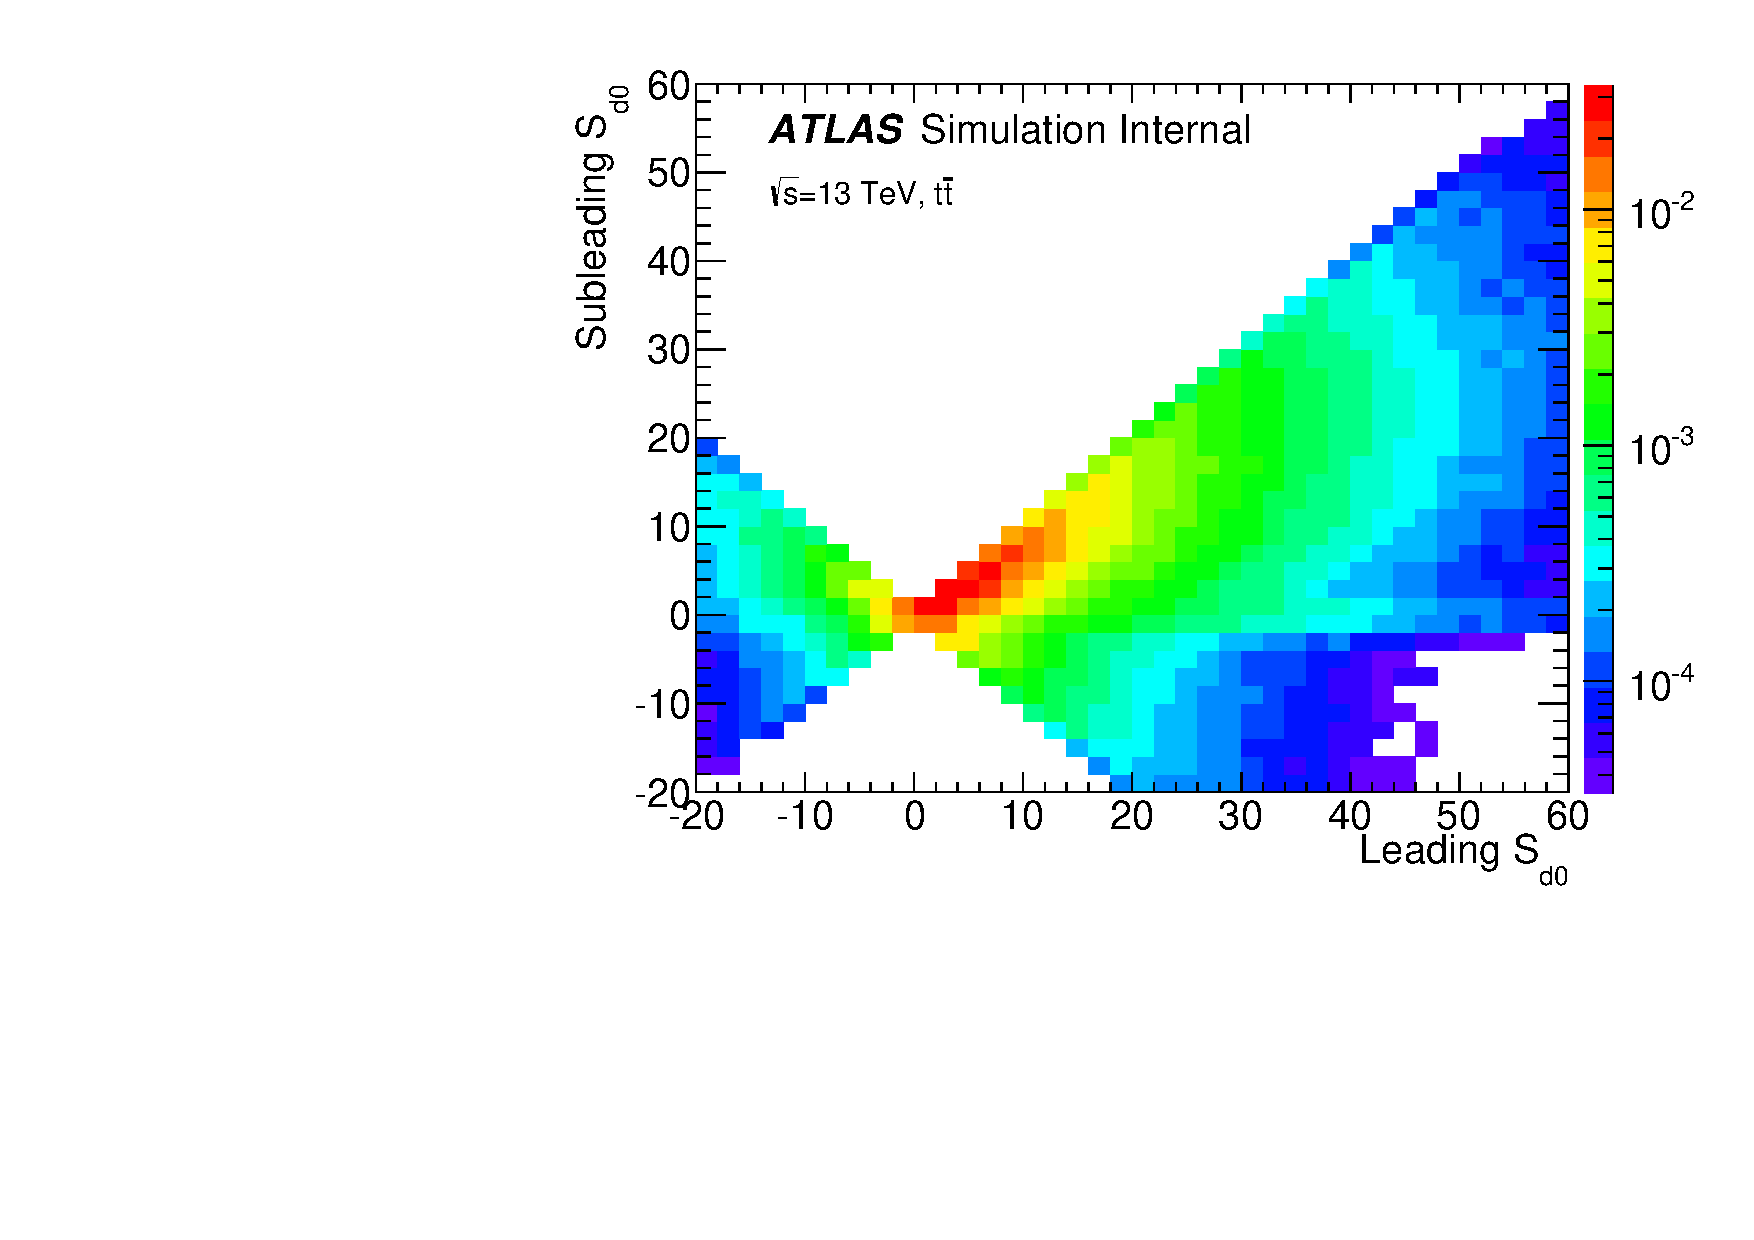
\includegraphics[width=0.48\textwidth]{figures/RNN/Sd0_2d_B.pdf}
 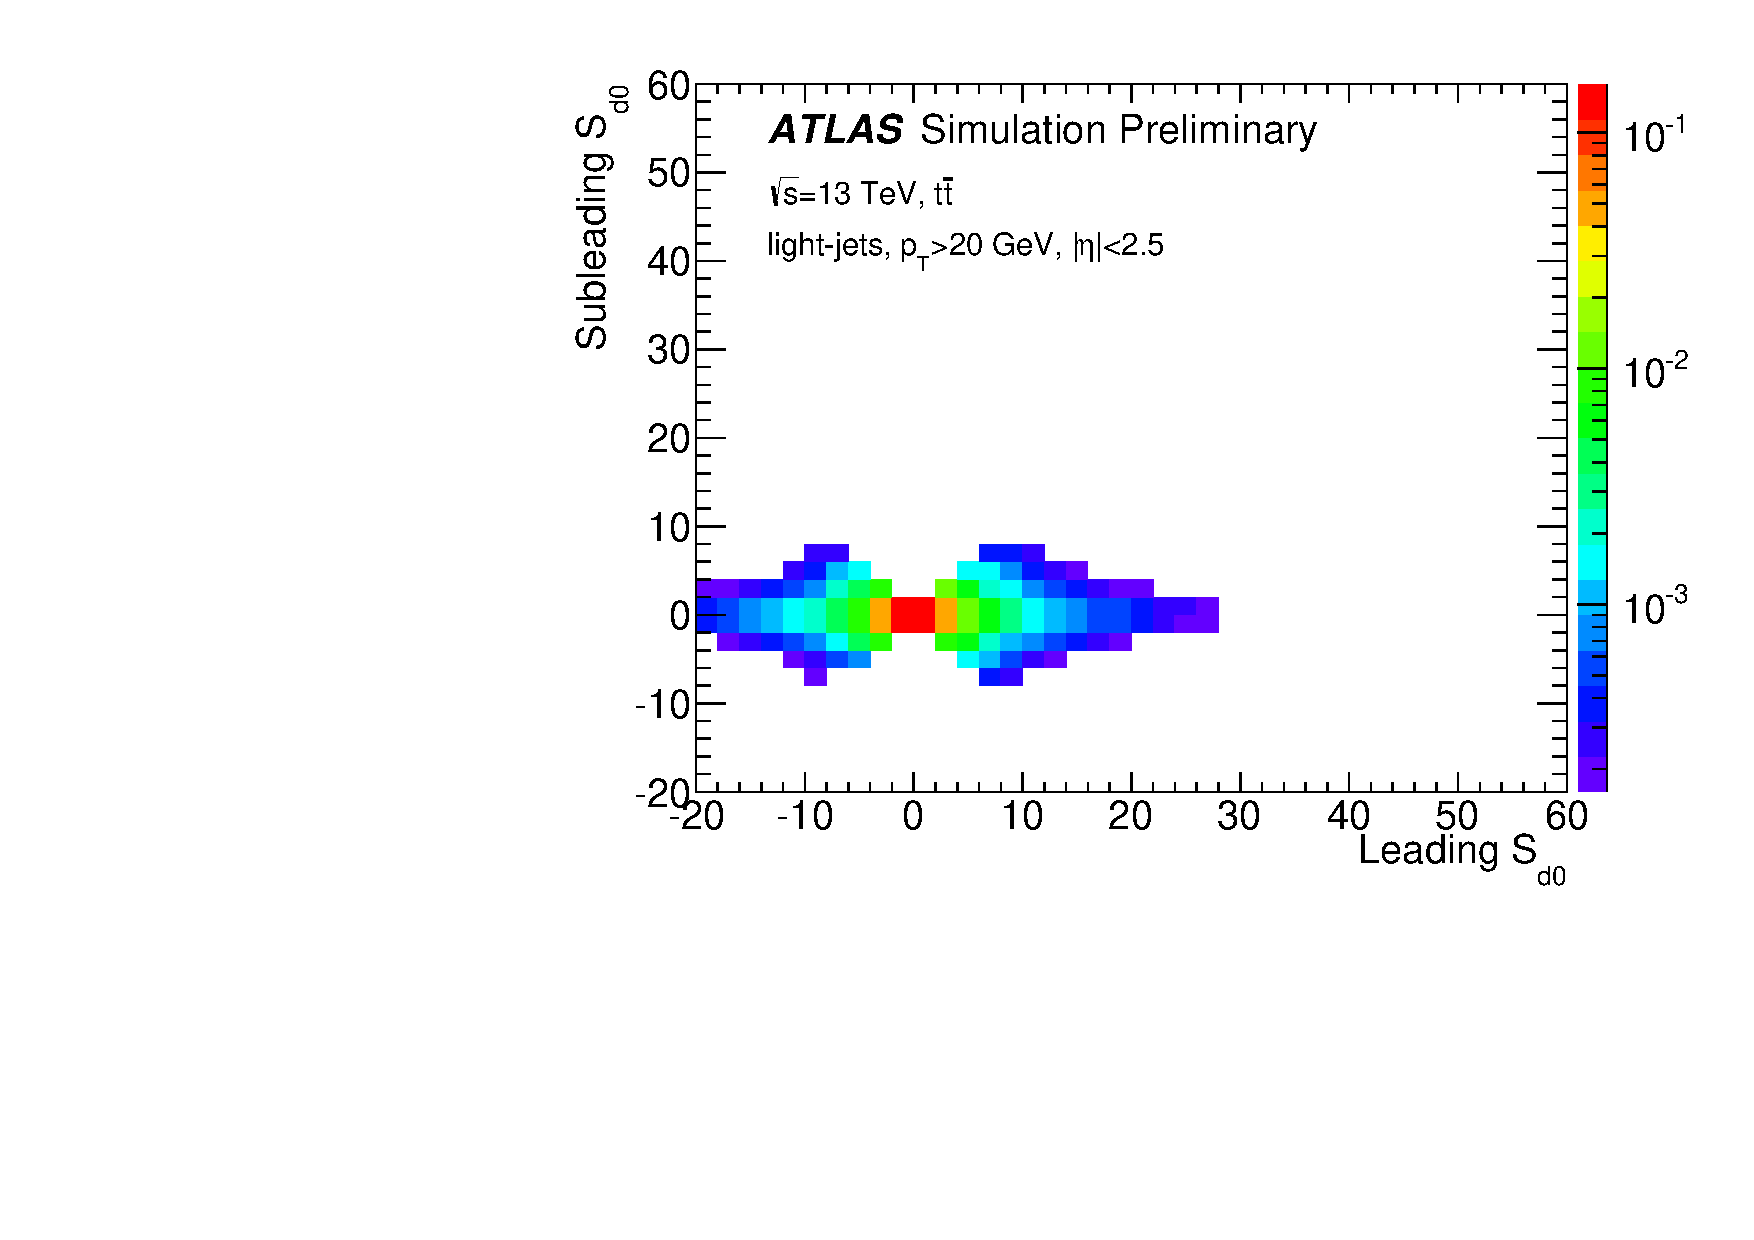
\includegraphics[width=0.48\textwidth]{figures/RNN/Sd0_2d_L.pdf}
\caption{The distribution of the \sdip for the leading and subleading $|\sdip|$ significance track in $b$-jets (left) and light jets (right). }
  \label{fig:ip_corr}
\end{figure}


The baseline \textit{IP3D} $b$-tagging algorithm, uses 3D likelihood templates in $\sdip$, $\szip$, and a track categorization to compute three per-flavor conditional likelihoods, $p_b$, $p_c$, and $p_{\textrm{light}}$. These likelihood templates are derived from histograms with 35 bins in $\sdip$, 20 bins in $\szip$, and 14 bins in track category, where each category corresponds to a different track quality~\cite{ATL-PHYS-PUB-2015-022}. Direct estimate of the joint probability distribution of these three variables is not possible, as the joint distribution has a total bin count of $35 \times 20 \times 14 \times 3 = 29,400$ if we want to maintain the same resolution as for the marginal distribution of each variable.In addition, extending the template to account for additional kinematic variables and the variable number of tracks within the jet is even more computationally expensive, as the number of template bins grows exponentially.

To overcome this difficulty, the \textit{IP3D} algorithm made the assumption that is that the per-track flavor conditional likelihood can be computed independent of the other tracks in the jet.  Such a likelihood model does not take into account correlations amongst track parameters, and the method of building templates to define likelihoods requires large sample sizes. Technicially, the \textit{IP3D} algorithm adopts a Naive Bayes estimate was made, the likelihood of a jet being of a given flavour is computed as the product of the per-track likelihoods which are in turn estimated by the product of per-track per-variable likelihohods . The \textit{IP3D} discriminant is built from the conditional log-likelihood ratio, $\textrm{IP3D}=\ln \prod_{i \in \textrm{tracks}} p_b^i / p_{\textrm{light}}^i$. 

\subsection{Recurrent Networks}

Recurrent Neural Networks are used to learn patterns in variable-length ordered inputs features~\cite{ref:RNNthesis, dlbook}. In contrast to regular multi-layer perceptrons, the forward pass equation of the hidden RNN units has in addition an activation from itself from the previous time-stamp: $O^t_l = A( W_i x_t + W_{l,l'} O^{t-1}_{l'})$, where $O$ is the output of the $l^{\text{th}}$ hidden layer's $t^{\text{th}}$ time-stamp; $A$ is the activation function, usually in the form of sigmoid function, tanh and etc.; $W_i$ are the network input weights, which is common to multi-layer perceptrons; $W_{l,l'}$ are the recurrent weights which are unique to RNNs. In this way a recurrent cell is able to reduce a sequence of arbitrary length to a fixed number of variables, which can then be processed by a traditional feed-forward network. The cell level illustration for a one-layer RNN is shown in Fig.\ref{fig:rnn_ilustration}.

\begin{figure}[htbp]
  \centering
   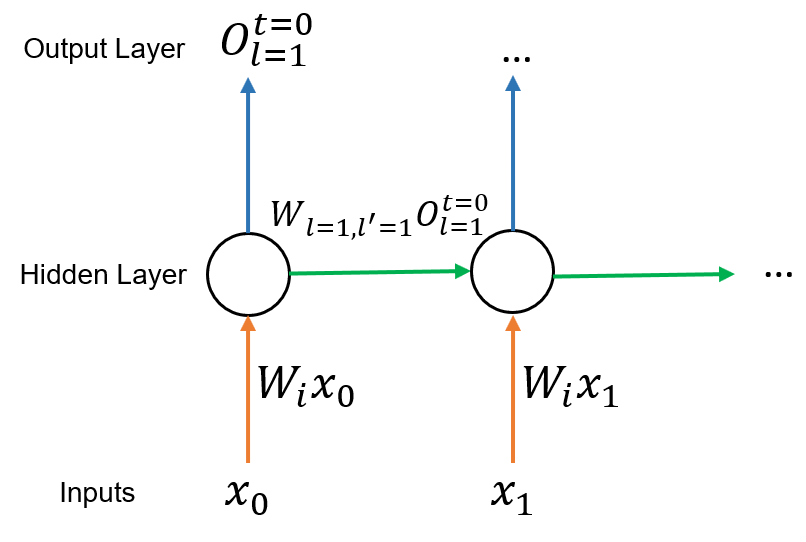
\includegraphics[width=0.5\textwidth]{figures/RNN/RNNIlustration.png}
\caption{Cell level illustration for a one-layer unrolled RNN}
  \label{fig:rnn_ilustration}
\end{figure}


%The fundamental unit of an RNN is a cell encapsulating an internal state vector. As the first step of processing any given sequence (in this case the tracks in a jet), the internal state is initialized to zero. At each step in the sequence, the cell is handed a fixed number of inputs (in this case the parameters that describe one track). These parameters are combined with the \emph{current} internal state in order to compute a \emph{new} internal state based on a set of rules which are tuned in the training phase. At the end of the sequence the cell's internal state serves as a fixed-dimensional representation of the entire sequence. 

It is not difficult to notice that, given a long input sequence, the derivative of the loss function with respect to the RNN weights will involve multiplicative terms which are the weights to the order of the length of the input sequence. Because of these terms, the gradient would likely explode or vanish~\cite{hochreiter1991untersuchungen,Bengio:1994:LLD:2325857.2328340,DBLP:journals/corr/abs-1211-5063}. In this work, a special type of RNN cell called Long Short-Term Memory (LSTM)~\cite{ref:LSTM} units are used to mitigate the vanishing and exploding gradients problem. This special kind of recurrent units employ different internal gating mechanisms to modify the cell state in order to balance and regulate the relative importance of long-term and short-term information as shown in Fig.\ref{fig:lstm_cell}. 


\begin{figure}[htbp]
  \centering
   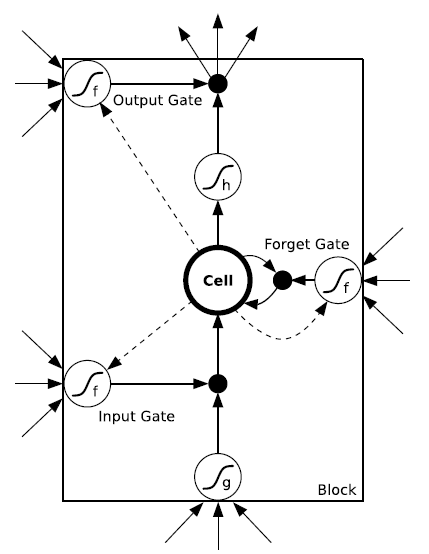
\includegraphics[width=0.5\textwidth]{figures/RNN/LSTM.png}
\caption{Illustration of LSTM RNN cell \cite{ref:RNNthesis}}
  \label{fig:lstm_cell}
\end{figure}
